% p35-operator-representable-over-a-cpo.tex
%
% Source: Carl A. Gunter and Dana S. Scott, "Semantic Domains".
%   physical page 35 of ScottDomains/papers/Gunter Scott 1990.pdf
%   printed page 34
%   section 7.1, "Solving domain equations with closures."
%   unnamed in the paper; introduced by this sentence:
%
%   "Definition: Let us say that an operator F on cpo's is representable over
%    a cpo U if and only if there is a continuous function R_F which completes
%    the following diagram (up to isomorphism):"
%
%   and read off immediately after by:  "i.e. im(R_F(r)) = F(im(r)) for every
%   closure r."
%
% What the diagram says: a universal property.  The solid arrows are the data
% the paper already has — the operator F on cpo's, and the map im from finitary
% closures on U to the cpo's they cut out.  The dashed arrow R_F is the map
% whose existence is being asserted, and the definition is that the square
% commutes up to isomorphism.  Solid versus dashed is the whole content; do not
% flatten it.  Theorem 21 on the same page is what the property buys: if F is
% representable over U then F has a fixed point, by taking a fixed point of R_F
% in the cpo Fc(U).
%
% Geometry: measured from the page, not idealized.  A 300 dpi crop of the
% region (candidate row "35 232 311 298 511" of
% analyses/diagram-candidates.2026-0808-10:32.orchestrator.log) puts the square
% at 474 x 236 px, i.e. 113.8 x 56.6 pt, so 4 cm x 2 cm here reproduces the
% paper's own size to within 1 percent at 28.45 pt per cm.
%
% Note: the arrow glyphs of this figure survive in the PDF, unlike the
% connecting lines of Figure 4 on page 44 — the arrows are ordinary math-font
% glyphs, whereas Figure 4's lines were picture-mode rules that the Paper
% Capture rebuild dropped.

\documentclass[border=6pt]{standalone}
\usepackage{tikz}
\begin{document}
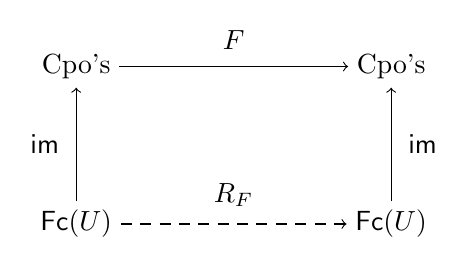
\begin{tikzpicture}[
  x=1cm, y=1cm,
  every node/.style={inner sep=1pt},
  open/.style={circle, draw, fill=white, minimum size=4pt, inner sep=0pt},
  solid/.style={circle, draw, fill=black, minimum size=5pt, inner sep=0pt},
  edge/.style={draw, line width=0.4pt},
  obj/.style={inner sep=3pt},
  arrow/.style={draw, line width=0.4pt, ->},
  darrow/.style={draw, line width=0.4pt, ->, dash pattern=on 4pt off 3pt}]

  % ---- objects ------------------------------------------------------------
  \node[obj] (TL) at (0,2) {Cpo's};
  \node[obj] (TR) at (4,2) {Cpo's};
  \node[obj] (BL) at (0,0) {$\mathsf{Fc}(U)$};
  \node[obj] (BR) at (4,0) {$\mathsf{Fc}(U)$};

  % ---- arrows -------------------------------------------------------------
  % label offsets are the paper's: 11 pt clear of the arrow, measured off a
  % 300 dpi crop (4.167 px/pt) as 46-48 px from label centre to arrow.
  \draw[arrow]  (TL) -- node[above=5pt] {$F$}   (TR);
  \draw[darrow] (BL) -- node[above=5pt] {$R_F$} (BR);
  \draw[arrow]  (BL) -- node[left=5pt]  {$\mathsf{im}$} (TL);
  \draw[arrow]  (BR) -- node[right=5pt] {$\mathsf{im}$} (TR);
\end{tikzpicture}
\end{document}
